\documentclass{article}
\usepackage{amsmath}
\usepackage{tikz}
\usepackage{geometry}
\usepackage{enumerate}
\renewcommand{\labelenumi}{(\alph{enumi})}
\renewcommand{\labelenumii}{(\roman{enumii})}
\geometry{verbose,letterpaper,tmargin=2cm,bmargin=2cm,lmargin=2cm,rmargin=2cm}

\title{CS181: Bayesian Networks and HMMs}
\author{Danny Zhu \& Tianhui Cai}
\let\b\mathbf

\begin{document}
\maketitle

\section*{Problem 1}
\begin{center}
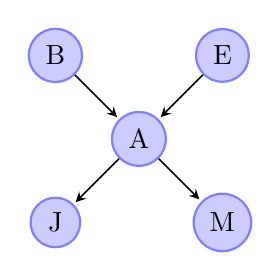
\begin{tikzpicture}[->,semithick,>=stealth,node distance=1.5cm,shorten >=1pt]
  \tikzstyle{state}=[circle,draw=blue!50,fill=blue!20,thick]
  \node [state] (B) {B};
  \node [state] (A) [below right of=B] {A};
  \node [state] (E) [above right of=A] {E};
  \node [state] (J) [below left of=A] {J};
  \node [state] (M) [below right of=A] {M};

  \path (B) edge (A)
        (E) edge (A)
        (A) edge (J)
            edge (M);
\end{tikzpicture}
\end{center}

\begin{enumerate}[(a)]
\item \textit{Let $S$ be the set of all nodes in the network. Using the idea 
  of $d$-separation, for each pair of nodes $U,V\in S$, list the subsets of
  $S\setminus \{U,V\}$ that when observed would render $U,V$ independent.}

  \begin{tabular}{|c|c|}
  \hline
  Node pair $(U,V)$ & $S'\subset S\setminus \{U,V\},I(U,V|S')$ \\
  \hline
  $(B, A)$ & Impossible \\
  $(B, E)$ & $\emptyset$ \\
  $(B, J)$ & $A$ \\ 
  $(B, M)$ & $A$ \\
  $(E, A)$ & Impossible \\
  $(E, J)$ & $A$ \\
  $(E, M)$ & $A$ \\
  $(A, J)$ & Impossible \\
  $(A, M)$ & Impossible \\
  $(J, M)$ & $A$ \\
  \hline
  \end{tabular}

\item \textit{Build another Bayesian network that has the same independence 
  properties, using variable order $M,J,A,B,E$.}

  The process is to consider $M,J,A,B,E$ in order and for each node $N_i$ to find 
  the minimal set of nodes $Pa(N_i)$ such that $P(N_i|N_1,\ldots,N_{i-1})=P(N_i|Pa(N_i))$. 

  Doing this iteratively, $P(M)=P(M)$; $P(J|M)=P(J|M)$; $P(A|M,J)=P(A|M)$; 
  $P(B|M,J,A)=P(B|A)$; $P(E|M,J,A,B)=P(E|A)$. Hence we get the following diagram:

\begin{center}
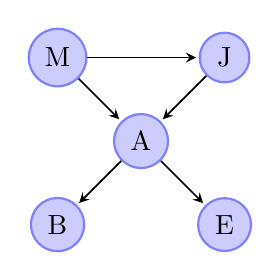
\begin{tikzpicture}[->,semithick,>=stealth,node distance=1.5cm,shorten >=1pt]
  \tikzstyle{state}=[circle,draw=blue!50,fill=blue!20,thick]
  \node [state] (B) {M};
  \node [state] (A) [below right of=B] {A};
  \node [state] (E) [above right of=A] {J};
  \node [state] (J) [below left of=A] {B};
  \node [state] (M) [below right of=A] {E};

  \path (B) edge (A)
            edge (E)
        (E) edge (A)
        (A) edge (J)
            edge (M);
\end{tikzpicture}
\end{center}
\item \textit{How may parameters are there in the BN in (a) and the BN in (b)?}

  (a): $(k-1)+(k-1)+k^2(k-1)+k(k-1)+k(k-1)$.

  (b): $(k-1)+k(k-1)+k^2(k-1)+k(k-1)+k(k-1)$.   

  \textit{Give there reasons why the BN in (a) is preferred over the BN in (b).}

  \begin{enumerate} 
  \item Fewer parameters means less storage.
  \item Fewer parameters means better sampling of data. 
  \item No cycles $\rightarrow$ polytree $\rightarrow$ optimal elimination order.
  \end{enumerate}

\end{enumerate}

\section{Problem 2}
\begin{enumerate}[(a)]
\item \textit{Suppose the driver does not detect a cop and the traffic is slow. 
  Use variable elimination to determine}

  TODO: I'm not sure what variable elimination has to do with anything. 

  \begin{enumerate}
  \item \textit{The probability of being late when the driver decides to speed 
    and when the driver decides not to speed}

    If the driver speeds, we obtain probability 
    $$1-\left[P(OT=T|Ticket=T,S=T)P(Ticket=T|S=T)+P(OT=T|Ticket=F,S=T)P(Ticket=F|S=T)\right]$$
    $$=1-\left[0\cdot P(Ticket=T|S=T,SC=F,ST=T)+0.9\cdot P(Ticket=F|S=T,SC=F,ST=T)=1-0.9\cdot (1-0.477)\right]=0.502$$
    using results from the second part of the problem.

   If the driver doesn't speed, we obtain probability
   $$1-\left[P(OT=T|Ticket=T,S=F)P(Ticket=T|S=F)+P(OT=T|Ticket=F,S=F)P(Ticket=F|S=F)\right]$$
   $$=1-\left[0\cdot P(Ticket=T|S=F,SC=F,ST=T)+0.1\cdot P(Ticket=F|S=F,SC=F,ST=T)\right]$$
   $$=1-0.1\cdot (1)=0.9$$
 

  \item \textit{The probability of getting a ticket when the driver decides to 
    speed and when the driver decides not to speed}

    If the driver speeds, we obtain probability
    $$P(Ticket=T|SC=F,S=T,ST=T)$$
    $$=P(Ticket=T|C=T,S=T,ST=T)P(C=T|SC=F,S=T,ST=T)+P(Ticket=T|C=F,S=T,ST=T)P(C=F|SC=F,S=T,ST=T)$$
    $$=0.5\cdot P(C=T|SC=F,S=T,ST=T)+0\cdot P(C=F|SC=F,S=T,ST=T)$$
    We need to find $P(C=F|SC=F,S=T,ST=T)$. By local independence of the BN, this equals $P(C=F|SC=F,ST=T)$. 
    This equals, by using local independence of SC and ST given C,
    \begin{align*}
    \frac{P(C=F,SC=F,ST=T)}{P(SC=F,ST=T)} & =\frac{P(SC=F,ST=T|C=F)P(C=F)}{P(SC=F,ST=T|C=F)P(C=F)+P(SC=F,ST=T|C=T)P(C=T)}\\
      & =\frac{P(SC=F|C=F)P(ST=T|C=F)P(C=F)}{P(SC=F|C=F)P(ST=T|C=F)P(C=F)+P(SC|C=T)P(ST=T|C=T)P(C=T)}\\
      & =\frac{1\cdot 0.3\cdot 0.9}{1\cdot 0.3\cdot 0.9+0.4\cdot 0.8\cdot 0.1} = 0.894\\
    \end{align*}
    Hence the probability of getting a ticket is, as before, $$0.5\cdot 0.894=0.447$$

    If the driver doesn't speed, we get
    $$P(Ticket=T,SC=F,S=F,ST=T)=P(Ticket=T|C=T,S=F,ST=T)P(C=T|SC=F,S=F,ST=T)+P(Ticket=T|C=F,S=F,ST=T)P(C=F|SC=F,S=F,ST=T)
      =0\cdot \cdot P(C=T|SC=F,S=T,ST=T)+0\cdot P(C=F|SC=F,S=T,ST=T)=0$$

  \item \textit{Suppose the cost of a ticket is \$150, and the cost of arriving 
    late is \$10. What is the expected utility of speeding and not speeding?
    What would be the optimal decision?}

   Speeding: $-\left[ 150\cdot 0.477 +10\cdot 0.502\right]=-76.57$ 

   Not speeding: $-\left[150\cdot 0+10\cdot 0.9\right]=-9$

   Clearly we should not speed. 
  \end{enumerate}
\end{enumerate}

\end{document}
